\documentclass[twoside]{article}

% We add packages, macros here:
%!TEX root =  lec-template.tex
\usepackage{lmodern}
\usepackage[english]{babel}
\usepackage{latexsym}
\usepackage{amsmath}
\usepackage{mathrsfs}
\usepackage{amssymb}
\usepackage{mathtools}
\usepackage[inline,shortlabels]{enumitem} % we prefer enumitem because of its margin adjustment caps
\usepackage{bm}
\usepackage{datetime}
\usepackage[table,xcdraw]{xcolor}
\usepackage{accents}
\usepackage{tikz}
\usepackage{listings}
\usepackage{mdframed}
\usepackage{pgfplots}
\usepackage{pgfplotstable}
\usepackage[boxed]{algorithm}
\usepackage{algpseudocode}
\usepackage{dsfont}
\usepackage{color}
\usepackage{colortbl}
\usepackage{pifont}
\usepackage[bf,font=small,singlelinecheck=off]{caption}
\usepackage{microtype} % improved spacing between words for easier reading
\usepackage{float}
\usepackage{xfrac} % sfrac
\usepackage{xspace}

\linespread{1.1}


\usepackage[textsize=tiny]{todonotes}
\makeatletter
\renewcommand{\todo}[2][]{\@todo[#1]{#2}}
\makeatother

\setlength{\marginparwidth}{10ex}
\newcommand{\todoc}[2][]{\todo[size=\scriptsize,color=blue!20!white,#1]{Csaba: #2}}
\newcommand{\todoj}[2][]{\todo[size=\scriptsize,color=red!20!white,#1]{Jincheng: #2}}

\usepackage{hyperref}
\hypersetup{
    unicode=false,          % non-Latin characters in Acrobat�s bookmarks
    pdftoolbar=true,        % show Acrobat�s toolbar?
    pdfmenubar=true,        % show Acrobat�s menu?
    pdffitwindow=false,     % window fit to page when opened
    pdfstartview={FitH},    % fits the width of the page to the window
    pdftitle={},    % title
    pdfauthor={},     % author
    pdfsubject={Theory, Machine Learning, Lectures},   % subject of the document
    pdfcreator={},   % creator of the document
    pdfproducer={}, % producer of the document
    pdfkeywords={theory} {machine learning} {lecture notes} {CMPUT 654} {Fall 2023}, % list of keywords
    pdfnewwindow=true,      % links in new window
    colorlinks=true,       % false: boxed links; true: colored links
    linkcolor=blue,          % color of internal links (change box color with linkbordercolor)
    citecolor=blue,        % color of links to bibliography
    filecolor=magenta,      % color of file links
    urlcolor=cyan           % color of external links
}
\usepackage{amsthm}
\usepackage{times}
\usepackage{natbib}
\usepackage{nicefrac}
\usepackage{wrapfig}
\usepackage[capitalize]{cleveref}
\usepackage[nottoc,numbib]{tocbibind}

%\usepackage[bmargin=0.75in]{geometry}
\usepackage[margin=1.1in]{geometry}
\usepackage[normalem]{ulem}


%%%%%%%%%%%%%%%%%%%%%%%%%%%%%%%%
% HYPHENATION
%%%%%%%%%%%%%%%%%%%%%%%%%%%%%%%%

\pretolerance=5000
\tolerance=9000
\emergencystretch=0pt
\righthyphenmin=4
\lefthyphenmin=4


\bibliographystyle{plainnat}

\newcommand{\E}{\mathbb{E}}
\newcommand{\EE}[1]{\E[#1]}
\newcommand{\PP}{\mathbb{P}}
\newcommand{\Prob}[1]{\mathbb{P}(#1)}
\newcommand{\one}[1]{\mathbb{I}\{#1\}}
\newcommand{\Supp}{\operatorname{supp}}
\newcommand{\ip}[1]{\langle #1 \rangle}
\newcommand{\bip}[1]{\left\langle #1 \right\rangle}
\newcommand{\norm}[1]{\|#1\|}
\newcommand{\R}{\mathbb{R}}
\newcommand{\N}{\mathbb{N}}
\newcommand{\cA}{\mathcal{A}}
\newcommand{\cB}{\mathcal{B}}
\newcommand{\cC}{\mathcal{C}}
\newcommand{\cD}{\mathcal{D}}
\newcommand{\cE}{\mathcal{E}}
\newcommand{\cF}{\mathcal{F}}
\newcommand{\cG}{\mathcal{G}}
\newcommand{\cH}{\mathcal{H}}
\newcommand{\cK}{\mathcal{K}}
\newcommand{\cL}{\mathcal{L}}
\newcommand{\cN}{\mathcal{N}}
\newcommand{\cP}{\mathcal{P}}
\newcommand{\cQ}{\mathcal{Q}}
\newcommand{\cR}{\mathcal{R}}
\newcommand{\cS}{\mathcal{S}}
\newcommand{\sA}{\mathscr A}

\newcommand{\cM}{\mathcal{M}}
\newcommand{\cX}{\mathcal{X}}
\newcommand{\cY}{\mathcal{Y}}
\newcommand{\NN}{\mathbb{N}}
\newcommand{\RR}{\mathbb{R}}
\newcommand{\VV}[1]{\mathbb{V}[#1]}

\newcommand{\epsapp}{\epsilon}
\newcommand{\epssub}{\delta}

\DeclareMathOperator{\Range}{range}
\newcommand{\rows}{\operatorname{rows}}

\renewcommand{\epsilon}{\varepsilon}
\newcommand{\ceil}[1]{\left\lceil {#1} \right\rceil}
\newcommand{\floor}[1]{\left\lfloor {#1} \right\rfloor}
\newcommand{\ones}{\mathbf{1}}
\newcommand{\zeros}{\mathbf{0}}
\DeclareMathOperator*{\argmin}{arg\ min}
\DeclareMathOperator*{\argmax}{arg\ max}


\def\rvzero{{\mathbf{0}}}
\def\rvone{{\mathbf{1}}}

\def\identiymatrix{\mathbf{Id}}

\newcommand{\softmax}{\mathrm{softmax}}
\newcommand{\KL}{D_{\mathrm{KL}}}

% Graph
\def\gA{{\mathcal{A}}}
\def\gB{{\mathcal{B}}}
\def\gC{{\mathcal{C}}}
\def\gD{{\mathcal{D}}}
\def\gE{{\mathcal{E}}}
\def\gF{{\mathcal{F}}}
\def\gG{{\mathcal{G}}}
\def\gH{{\mathcal{H}}}
\def\gI{{\mathcal{I}}}
\def\gJ{{\mathcal{J}}}
\def\gK{{\mathcal{K}}}
\def\gL{{\mathcal{L}}}
\def\gM{{\mathcal{M}}}
\def\gN{{\mathcal{N}}}
\def\gO{{\mathcal{O}}}
\def\gP{{\mathcal{P}}}
\def\gQ{{\mathcal{Q}}}
\def\gR{{\mathcal{R}}}
\def\gS{{\mathcal{S}}}
\def\gT{{\mathcal{T}}}
\def\gU{{\mathcal{U}}}
\def\gV{{\mathcal{V}}}
\def\gW{{\mathcal{W}}}
\def\gX{{\mathcal{X}}}
\def\gY{{\mathcal{Y}}}
\def\gZ{{\mathcal{Z}}}

% Sets
\def\sA{{\mathbb{A}}}
\def\sB{{\mathbb{B}}}
\def\sC{{\mathbb{C}}}
\def\sD{{\mathbb{D}}}
% Don't use a set called E, because this would be the same as our symbol
% for expectation.
\def\sE{{\mathbb{E}}}
\def\sF{{\mathbb{F}}}
\def\sG{{\mathbb{G}}}
\def\sH{{\mathbb{H}}}
\def\sI{{\mathbb{I}}}
\def\sJ{{\mathbb{J}}}
\def\sK{{\mathbb{K}}}
\def\sL{{\mathbb{L}}}
\def\sM{{\mathbb{M}}}
\def\sN{{\mathbb{N}}}
\def\sO{{\mathbb{O}}}
\def\sP{{\mathbb{P}}}
\def\sQ{{\mathbb{Q}}}
\def\sR{{\mathbb{R}}}
\def\sS{{\mathbb{S}}}
\def\sT{{\mathbb{T}}}
\def\sU{{\mathbb{U}}}
\def\sV{{\mathbb{V}}}
\def\sW{{\mathbb{W}}}
\def\sX{{\mathbb{X}}}
\def\sY{{\mathbb{Y}}}
\def\sZ{{\mathbb{Z}}}

\newcommand{\dimE}{\mathrm{dim}_{\mathcal{E}}}
\DeclareMathOperator{\diam}{diam}


%%
%% ADD PACKAGES here:
%%
%
%\usepackage{amsmath,amsfonts,graphicx}
%
%
% The following commands set up the lecnum (lecture number)
% counter and make various numbering schemes work relative
% to the lecture number.
%

\newcounter{lecnum}
\renewcommand{\thepage}{\thelecnum-\arabic{page}}
\renewcommand{\thesection}{\thelecnum.\arabic{section}}
\renewcommand{\theequation}{\thelecnum.\arabic{equation}}
\renewcommand{\thefigure}{\thelecnum.\arabic{figure}}
\renewcommand{\thetable}{\thelecnum.\arabic{table}}


%
% The following macro is used to generate the header.
%
\newcommand{\lecture}[4]{
   \pagestyle{myheadings}
   \thispagestyle{plain}
   \newpage
   \setcounter{lecnum}{#1}
   \setcounter{page}{1}
   \noindent
   \begin{center}
   \framebox{
      \vbox{\vspace{2mm}
    \hbox to 6.28in { {\bf CMPUT 654 Fa 23: Theoretical Foundations of Machine Learning \hfill Fall 2023} }
       \vspace{4mm}
       \hbox to 6.28in { {\Large \hfill Lecture #1: #2  \hfill} }
       \vspace{2mm}
       \hbox to 6.28in { {\it Lecturer: #3 \hfill Scribes: #4} }
      \vspace{2mm}}
   }
   \end{center}
   \markboth{Lecture #1: #2}{Lecture #1: #2}

   \noindent {\bf Note}: {\it 
   \LaTeX\  template courtesy of UC Berkeley EECS dept. (\href{https://inst.eecs.berkeley.edu/~cs294-8/sp03/Materials/}{link} to directory)
   }

   \noindent {\bf Disclaimer}: {\it These notes have \underline{\textbf{not}} been subjected to the
   usual scrutiny reserved for formal publications. They may be
   distributed outside this class only with the permission of the
   Instructor.} \vspace*{4mm}
}
%
% Convention for citations is authors' initials followed by the year.
% For example, to cite a paper by Leighton and Maggs you would type
% \cite{LM89}, and to cite a paper by Strassen you would type \cite{S69}.
%%%%%%%%% (To avoid bibliography problems, for now we redefine the \cite command.)
%%%%%%%%% Also commands that create a suitable format for the reference list.
%%%%%%%%\renewcommand{\cite}[1]{[#1]}
%%%%%%%%\def\beginrefs{\begin{list}%
%%%%%%%%        {[\arabic{equation}]}{\usecounter{equation}
%%%%%%%%         \setlength{\leftmargin}{2.0truecm}\setlength{\labelsep}{0.4truecm}%
%%%%%%%%         \setlength{\labelwidth}{1.6truecm}}}
%%%%%%%%\def\endrefs{\end{list}}
%%%%%%%%\def\bibentry#1{\item[\hbox{[#1]}]}

%Use this command for a figure; it puts a figure in wherever you want it.
%usage: \fig{NUMBER}{SPACE-IN-INCHES}{CAPTION}
\newcommand{\fig}[3]{
			\vspace{#2}
			\begin{center}
			Figure \thelecnum.#1:~#3
			\end{center}
	}
% Use these for theorems, lemmas, proofs, etc.

%!TEX root =  lec-template.tex
%%%%%%%%%%%%%%%%%%%%%%%%%%%%%%%%
% THEOREMS
%%%%%%%%%%%%%%%%%%%%%%%%%%%%%%%%
\theoremstyle{plain}
\newtheorem{theorem}{Theorem}[lecnum]
\newtheorem{claim}[theorem]{Claim}
\newtheorem{proposition}[theorem]{Proposition}
\newtheorem{lemma}[theorem]{Lemma}
\newtheorem{corollary}[theorem]{Corollary}
\newtheorem{example}[theorem]{Example}
\theoremstyle{definition}
\newtheorem{definition}[theorem]{Definition}
\newtheorem{assumption}[theorem]{Assumption}
\newtheorem{remark}[theorem]{Remark}
\newtheorem{exercise}[theorem]{Exercise}
\theoremstyle{remark}


%\newtheorem{theorem}{Theorem}[lecnum]
%\newtheorem{lemma}[theorem]{Lemma}
%\newtheorem{proposition}[theorem]{Proposition}
%\newtheorem{claim}[theorem]{Claim}
%\newtheorem{corollary}[theorem]{Corollary}
%\newtheorem{definition}[theorem]{Definition}
%\newenvironment{proof}{{\bf Proof:}}{\hfill\rule{2mm}{2mm}}

% **** IF YOU WANT TO DEFINE ADDITIONAL MACROS FOR YOURSELF, PUT THEM HERE:

\newcommand\myE{\mathbb{E}}

\begin{document}
%FILL IN THE RIGHT INFO.
%\lecture{**LECTURE-NUMBER**}{**DATE**}{**LECTURER**}{**SCRIBE**}
\lecture{4}{September 14}{Csaba Szepesv\'ari}{Zixin Zhong}
%\footnotetext{These notes are partially based on those of Nigel Mansell.}

% **** YOUR NOTES GO HERE:

% Some general latex examples and examples making use of the
% macros follow.  
%**** IN GENERAL, BE BRIEF. LONG SCRIBE NOTES, NO MATTER HOW WELL WRITTEN,
%**** ARE NEVER READ BY ANYBODY.


\section{Outline}

\begin{enumerate}
    \item Concentration inequalities:
        \\ Chernoff's inequality, multiplicative Chernoff's inequality; Bernett's inequality, Bernstein inequality
    \item PAC-learning:
        \\ PAC learnability based on `fitness'/union bounds
\end{enumerate}

\section{Concentration inequalities}

\begin{theorem}[Chernoff's Inequality]
    Let $X_1,\ldots, X_n\in [0,1]$ be i.i.d.\ random variables, $\bar{X}_n=\frac{1}{n}(X_1+\ldots+X_n)$, $\mu = \mathbb{E}X_1$. We have
    \begin{enumerate}[(a)]
        \item  $\forall \delta\in (0,1)$, with probability $1-\delta$,
    \begin{align*}
        \bar{X}_n \le \mu + \sqrt{\frac{\log(1/\delta)}{2n}};
    \end{align*}
        \item $\forall \delta\in (0,1)$, with probability $1-\delta$,
    \begin{align*}
        \bar{X}_n \ge \mu - \sqrt{\frac{\log(1/\delta)}{2n}}.
    \end{align*}
    \end{enumerate}
   
\end{theorem}

\begin{proof}
    Since $X_1\in[a,b]$ implies that $X_1$ is $\sigma(X_1)$-SG with $\sigma(X_1)= \frac{b-a}{n}$, $X_1\in[0,1]$ indicates that
    \begin{align*}
        \sigma(\bar{X}_n) = \frac{ \sigma(X_1) }{ \sqrt{n} } = \frac{1}{ 2\sqrt{n} }.
    \end{align*}
    Applying this fact with Hoeffding inequality, the Chernoff's inequality is proven.
\end{proof}

\begin{theorem}[Multiplicative Chernoff's Inequality]
    Let $X_1,\ldots, X_n\in [0,1]$ be i.i.d.\ random variables, $\bar{X}_n=\frac{1}{n}(X_1+\ldots+X_n)$, $\mu = \mathbb{E}X_1$. We have
    \begin{enumerate}[(a)]
        \item $\forall \delta\in (0,1)$, with probability $1-\delta$,
    \begin{align*}
        \bar{X}_n \le \mu + \sqrt{\frac{2\mu\log(1/\delta)}{n}}+\frac{1}{3n};  
    \end{align*}
    \item $\forall \delta\in (0,1)$, with probability $1-\delta$,
    \begin{align*}
        \bar{X}_n \ge \mu - \sqrt{\frac{2\mu\log(1/\delta)}{n}}.    \qquad\qquad \text{(*)}
    \end{align*}
    \end{enumerate}
  
\end{theorem}

\begin{remark} \mbox{}
    \begin{enumerate}[(a)]
        \item How big can $\mu$ be? 
            \\ By (*): $\mu \le \bar{X}_n + \sqrt{\frac{2\mu\log(1/\delta)}{n}}.$
        \item Let
            \begin{align*}
                f(a,c)=\max\{ u: u\le a + \sqrt{u\cdot c} \}, \text{ where } a= \bar{X}_n,\ c=\frac{2 \log(1/\delta)}{n}.
            \end{align*}
            Then
            \begin{align*}
                & \mu + \frac{ \log(1/\delta) }{ 2 n } \ge \sqrt{ \frac{ 2 \mu \log(1/\delta) }{n} } \text{ and equality holds when } \mu = \frac{ \log(1/\delta) }{ 2 n },\\
                \Rightarrow & \inf_{0<\gamma <1} \gamma \mu +   \frac{ \log(1/\delta) }{ 2 \gamma n } =  \sqrt{ \frac{ 2 \mu \log(1/\delta) }{n} },  \\
                \Rightarrow 
                & \mu - \sqrt{\frac{2\mu\log(1/\delta)}{n}} = \sup_{0< \gamma<1} (1-\gamma) \mu - \frac{\log(1/\delta)}{2\gamma n} .
            \end{align*}
            Let $\gamma =1/2$, then with (*) we have
            \begin{align*}
                \bar{X}_n \ge \frac{ \mu }{2} - \frac{\log(1/\delta)}{ n }.
            \end{align*}
            \vspace*{-1em}
            \begin{figure}[H]
                \centering
                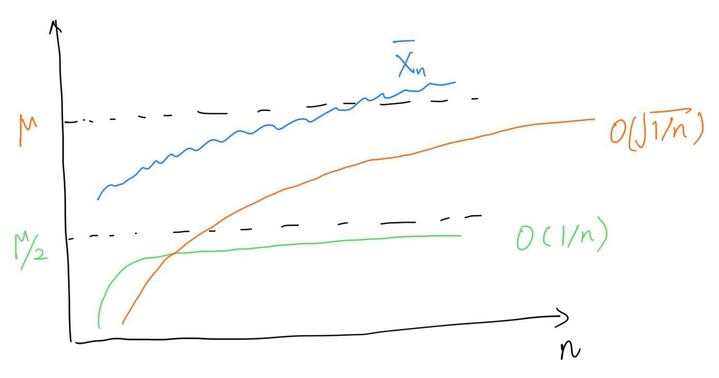
\includegraphics[width=0.5\textwidth]{draw - lec04.jpg}
                \caption{Example: set $\gamma=1/2$.}
                \label{fig:enter-label}
            \end{figure}
        \item When we apply $\gamma$ that does not maximize the term $(1-\gamma) \mu - \frac{\log(1/\delta)}{2\gamma n}$, we cannot claim that we get a better `convergence' rate, because when $n\rightarrow \infty$, $ (1-\gamma) \mu - \frac{\log(1/\delta)}{2\gamma n}$ and $\bar{X}_n$ converges to different values. In detail, $\bar{X}_n$ converges to $\mu$ regardless of the value of $\gamma$, and $(1-\gamma) \mu - \frac{\log(1/\delta)}{2\gamma n}$ converges to $(1-\gamma)\mu\ne \mu$ when $0<\gamma<1$.
        \\
        To say something about the convergence of $\bar{X}_n$, we need to have the coefficient of $\mu$ be $1$.
    \end{enumerate}
    
\end{remark}

\begin{theorem}[Bernett's Inequality]
    Let $X_1,\ldots, X_n$ be i.i.d.\ random variables. Set $\bar{X}_n=\frac{1}{n}(X_1+\ldots+X_n)$ and $\mu = \mathbb{E}X_1$.  If $X_1-\mu \le b$, with probability $1-\delta$, we have
    \begin{align*}
        \bar{X}_n \le \mu + \sqrt{ \frac{ 2 \Var(X_1) \log(1/\delta) }{n} } + \frac{b}{3n}.
    \end{align*}
    
\end{theorem}

\section{PAC-learning (L. Valiant)}

Let function  $f_*: \{0,1\}^d \rightarrow \{0,1\}$, $ X_1, X_2, \ldots, X_n \in \{0,1\}^d := \underline{2}^d$ be i.i.d.\ random variables drawn from distribution $P_X$, data set $D_n=\{ \left( X_1, f_*(X_1)\right), \ldots, \left( X_n, f_*(X_n)\right) \}$.

Let $f_* \in \mathcal{F} \subset \underline{2}^{ \underline{2}^d } $ and $f \in \underline{2}^{ \underline{2}^d } $, $P_X^{f_*}:= P(X_1, f_*{X_1})$, and 
\begin{align*}
    & L(f) = \mathbb{P} \left( f(X) \ne f_*(X) \right) = L( P_X^{f_*} ,f ),\\
    & l: \underline{2} \times \underline{2} \rightarrow \underline{2}, \quad l(y,y') = \mathbf{1}(y\ne y'),\\
    & L( P_X^{f_*},f  ) = \int P(\mathrm{d}x, \mathrm{d}y) \ l( f(x),y ).
\end{align*}

\begin{definition}[PAC-Learning]
    Fix $\mathcal{C} = (\mathcal{C}_d)_{d\ge 1}$, where $\mathcal{C}_d \subset \underline{2}^{\underline{2}^d }$. $\mathcal{C}$ is \textbf{PAC-learnable (\underline{P}roabably \underline{A}pproximately \underline{C}orrectly)} if $\exists$ polynomial $p\in \mathbb{R}[x,y,z]$ and $\mathcal{A}= (\mathcal{A}_{n,d})_{n\ge 1, d\ge 1}$ where $\mathcal{A}_{n,d}:\left( \underline{2}^d\times \underline{2} \right)^n \rightarrow  \underline{2}^{ \underline{2}^d }$
    \begin{align*}
        \text{s.t.\quad }
        & \forall  \varepsilon \in (0,1), \ \delta \in(0,1), \ d\ge 1, \ P \in \mathcal{M}_1(\underline{2}^d),\  f_* \in \mathcal{C}_d,\\
        & n\ge \lceil p( 1/\varepsilon, 1/\delta, d )\rceil,\\
        & X_1,X_2,\ldots,X_n\sim P_X,\\
        & f_n = \mathcal{A}_{n,d} \left( \underbrace{\left( X_1, f_*(X_1)\right), \ldots, \left( X_n, f_*(X_n)\right)}_{D_n} \right),
    \end{align*}
    we have
    \begin{align*}
        \mathbb{P}\left( L\left( P_X^{f_*},f_n \right) \ge \varepsilon  \right) \le \delta.
    \end{align*}
    In other words, with probability $1-\delta$, $\mathbb{P} \left( f_n(X) \ne f_*(x) | D_n \right) \le \varepsilon$.
\end{definition} 

\begin{remark}
    \begin{enumerate}[(a)] 
        \item Example:
        \begin{align*}
            \mathcal{C}_{\text{AND}}^d= \left\{  f:   \underline{2}^d \rightarrow \underline{2}\ | \ \exists u \subset[d],\ \forall x\in \underline{2}^d: f(x) = \min_{j\in u} X_j \right\}.
        \end{align*}
        \item (i) $L(f_*)=0$. (ii) When $Y_i=f_*(X_i)$, there is \textbf{NO} noise and this will make learning \textbf{faster}.
    \end{enumerate}  
\end{remark}


\end{document}h
